% \section{Bayesian Analysis for Inference}
% We now analyze how retrieved experiences influence the model’s reasoning process during inference.
% From a Bayesian perspective, the output distribution of model $f_{\theta}$ on query $\tilde{X}$ conditioned on the retrieved experience $\tilde{R}$ can be formulated as:
% \begin{equation}
% \begin{aligned}
% p_{FL}(\tilde{Y}\mid \tilde{X}) &= p_\theta(\tilde{Y}\mid \tilde{X},\tilde{R}) = \frac{p_\theta(\tilde{X},\tilde{R}\mid \tilde{Y})p_\theta(\tilde{Y})}{p_\theta(\tilde{X},\tilde{R})}=\frac{p_\theta(\tilde{X}\mid \tilde{Y})p_\theta(\tilde{R}\mid \tilde{X},\tilde{Y})p_\theta(\tilde{Y})}{p_\theta(\tilde{X})p_\theta(\tilde{R}\mid \tilde{X})}\\
% &=p_\theta(\tilde{Y}\mid \tilde{X})\frac{p_\theta(\tilde{R}\mid \tilde{X},\tilde{Y})}{p_\theta(\tilde{R}\mid \tilde{X})}
% \end{aligned}
% \end{equation}
% Here, $p_{\theta}(\tilde{Y}\mid \tilde{X})$ denotes the model’s {prior belief}, $p_{\theta}(\tilde{R}\mid \tilde{X})$ is the {evidence normalizer}, and $p_{\theta}(\tilde{R}\mid \tilde{X},\tilde{Y})$ is the {empirical likelihood} reflecting the compatibility of $\tilde{R}$ with $(\tilde{X},\tilde{Y})$.

% Incorporating $\tilde{R}$ into inference thus performs a {Bayesian update} that refines and corrects the model’s prior. 
% Note that \method{} optimizes for experiences that best align with and facilitate optimal reasoning outcomes.  
% Consequently, if $\tilde{R}$ highly aligns with the correct reasoning $\tilde{Y}$, the likelihood $p_{\theta}(\tilde{R}\mid \tilde{X}, \tilde{Y})$ is large, amplifying the prior and increasing the posterior probability of the correct prediction. 
% Conversely, if $\tilde{R}$ conflicts with incorrect hypotheses, $p_{\theta}(\tilde{R}\mid \tilde{X}, \tilde{Y})$ becomes small, thereby suppressing less plausible alternatives. 
% In summary, \method{} can be interpreted as a posterior augmentation mechanism, 
% where external experience serves as weighted evidence that adaptively reshapes the model’s belief toward more accurate and confident reasoning.


\section{Experimental Details}
% \subsection{Math}

% \paragraph{AIME25 Setup.} The evaluation was extended to SOTA models, including Claude-Sonnet-4.5 and GPT-5. We adopted the hierarchical experience library architecture established for the math benchmark and defined three experimental arms: (1) Naive LLM, (2) ReAct, and (3) \method{}. To construct the experience library, we curated a training set of 50 reactions from the USPTO50k dataset, with performance assessed on a held-out test set of 100 reactions. The learning process was executed for one epoch at a temperature of 0.

% \paragraph{GSM8k Setup.} To assess the generality of our paradigm, we extend our evaluation to a broader spectrum of models with varying capabilities, including GPT-3.5-Turbo, GPT-4, and Llama-3.2. For GSM8k, the experience library was initialized to store high-level strategic suggestions. A new suggestion was incorporated into the library only if it demonstrably improved performance on the 7k training set. In this context, we compare two primary configurations: (1) Naive LLM (the baseline model) and (2) \method{} (the model augmented with our experience library). The learning process was executed for one epoch at a temperature of 0.

% \subsection{Chemistry}

% \paragraph{Main Results.} The results, summarized in Table~\ref{tab:main_table}, reveal the profound impact of \method{} in a specialized scientific domain. The baseline performance of the naive LLMs underscores the challenge: Claude-Sonnet-4.5 achieves only 20\% accuracy, while GPT-5 secures just 9\%, highlighting the significant limitations of applying frozen, generalist models to complex chemical tasks. In stark contrast, after learning from a minimal set of 50 examples, \method{} elevates the performance of Claude-Sonnet 4.5 to 30\%. This represents a 10\% absolute improvement and a 50\% relative gain. These findings demonstrate that our paradigm provides a highly efficient pathway for domain adaptation, enabling agents to acquire critical specialized knowledge without parameter modification.

% \paragraph{The Value of Distilled Experience.} To deconstruct the sources of this performance gain, we performed an ablation study comparing the naive LLM, the standard ReAct agent, and our full \method{} implementation. On USPTO50k, the ReAct framework alone provides a marginal benefit, increasing accuracy to 23\%—a 3\% absolute improvement over the naive baseline. However, the introduction of the experience library prompts a substantial leap in performance, with \method{} outperforming the ReAct-only agent by an additional 7\% absolute points (a 30.4\% relative improvement). This clearly isolates the distilled experience as the primary driver of the agent's enhanced capability.

% \paragraph{Analysis.} Across the three trajectories in Figure~\ref{fig:case_study}, both the naive LLM and vanilla ReAct agent converge on the same fundamental error: misidentifying the retrosynthetic disconnection point. Despite correctly parsing the product structure and recognizing the presence of a mesylate group, they prioritize N-alkylation as the synthetic pathway, targeting the $\mathrm{C{-}N}$ bond between the piperidine nitrogen and the ethyl mesylate side chain. This reflects a critical gap in domain-specific pattern recognition—while N-alkylation is indeed a common transformation, the sulfonate ester motif ($\mathrm{-O{-}SO_2{-}CH_3}$) is a canonical signature of alcohol activation, where the diagnostic $\mathrm{O{-}S}$ bond should be the primary disconnection target. In contrast, \method{} succeeds by injecting procedural knowledge: retrieved `Golden Method 7` provides an explicit template ($\mathrm{R{-}O{-}SO_2{-}CH_3} \rightarrow \mathrm{R{-}OH} + \mathrm{CS(=O)(=O)Cl}$) that overrides the flawed heuristic, while `Warning Method 7` enforces negative constraints. This dual scaffolding transforms the agent's reasoning from exploratory hypothesis testing into a deterministic, domain-grounded workflow, ensuring the correct disconnection.

% \paragraph{The Role of the Experience Library.} The experience library addresses a fundamental tension in deploying frozen LLMs for complex, real-world applications: the brittleness of emergent reasoning when confronted with domain-specific subtleties. While LLMs excel at generating plausible surface-level reasoning, they lack the mechanisms to enforce consistency between declarative knowledge (e.g., "mesylates are good leaving groups") and procedural execution (e.g., "disconnect the O-S bond"). The experience library functions as an externalized, evolvable knowledge substrate that bridges this gap. By distilling verified problem-solving episodes into reusable templates, invariants, and failure patterns, it provides the agent with structured priors that guide exploration without requiring gradient-based retraining. This approach preserves the generality of the frozen LLM while augmenting it with task-specific expertise—a form of compositional generalization where the base model supplies linguistic scaffolding and the memory supplies domain constraints. The experience library thereby acts not merely as a cache but as a procedural epistemology—a repository of "how to think" in a domain, enabling frozen LLMs to navigate the gap between their parametric knowledge and the structured reasoning required in scientific problem-solving.

\subsection{Biology}

% \subsubsection{Configuration}

\textbf{Protein Fitness Prediction} We apply \method{} on the task of Protein Fitness Prediction. Proteins play a fundamental role in sustaining cellular functions that underpin organismal survival, growth, and reproduction. The capacity of a protein to perform its biological function—typically referred to as protein fitness—is determined by its three-dimensional structure, which is ultimately encoded by its amino acid sequence. Recent advances in machine learning have enabled zero-shot protein fitness prediction by leveraging representations derived from protein sequences, structural information, and auxiliary biological signals such as multiple sequence alignments (MSAs). Despite the progress, the task remains far from being fully solved. First, the absolute correlation between predicted and experimentally validated fitness scores remains limited (e.g., approximately 0.52 for the current state-of-the-art on ProteinGym), not confidential enough when encountering newly-found data with mysterious fitness. Second, no existing model consistently outperforms all others across diverse protein families and functional categories, including activity, expression, binding affinity, stability, and organismal fitness.




\paragraph{Agentic Task Transformation.} Large language model (LLM) agents, without specialized pre-training on protein sequences or domain-specific fine-tuning, inherently lack detailed biochemical knowledge and cannot directly infer subtle mutational effects on protein function. However, these agents possess strong capabilities in reasoning, ranking, knowledge synthesis, and few-shot learning. This opens a new opportunity: rather than directly predicting fitness from sequence, agents can be tasked with meta-reasoning over predictions made by high-performing protein language models. Specifically, we reformulate protein fitness prediction as an agentic feature selection and fusion task, where the agent learns to identify, prioritize, and integrate salient features derived from existing regression-based models. Through this process, the agent proposes explicit, interpretable algorithms that capture the underlying relationships among predictive signals, transforming opaque model outputs into a more accurate and explainable fitness prediction framework tailored to each target protein.




% \textbf{Experience, Memory and Verifier} Given task above, we‘d like to clerify how elements of \method{} are implied from the same paradigm.

% In all, experience are extracted from 100 tiny experience set for each protein independently since there're various protein properties as protein function object. In result, we'll have structured memoies consist of 3 parts: 1) golden rules and failure cases when selecting important features i.e. score predicted by specific model such as ProSST ~\cite{li2024prosst}. 2) beneficial and deterious algorithm with agent's own decision. 3) meta-level self-concluded cognitive about how to improve selcting strategies and combinging algorithm.


% For fair comparation, two categories of \method{} system are constructed: 1) training-free model where training parameterized models are forbiddened and agent is unavailable to use any regression tools. 2) Regression-related model where a series of regression method are provided as tools through sk-learn package. 



\paragraph{Benchmark.} We conduct experiments using the ProteinGym benchmark, which serves both as the source for experience extraction and as the evaluation dataset. Protein targets included in this benchmark align with those defined in SaProt~\cite{su2023saprot}. To emulate realistic biological discovery scenarios where experimental data is scarce, we adopt an imbalanced data split for each protein: a small experience set consisting of only 100 sequences (on average 1.47\% of the available data), and a large out-of-distribution test set containing all remaining sequences. This design reflects practical constraints in protein engineering, where only a limited number of labeled mutations are known, while the vast majority of sequence space remains unexplored.


\begin{figure}[!t]
  \centering
  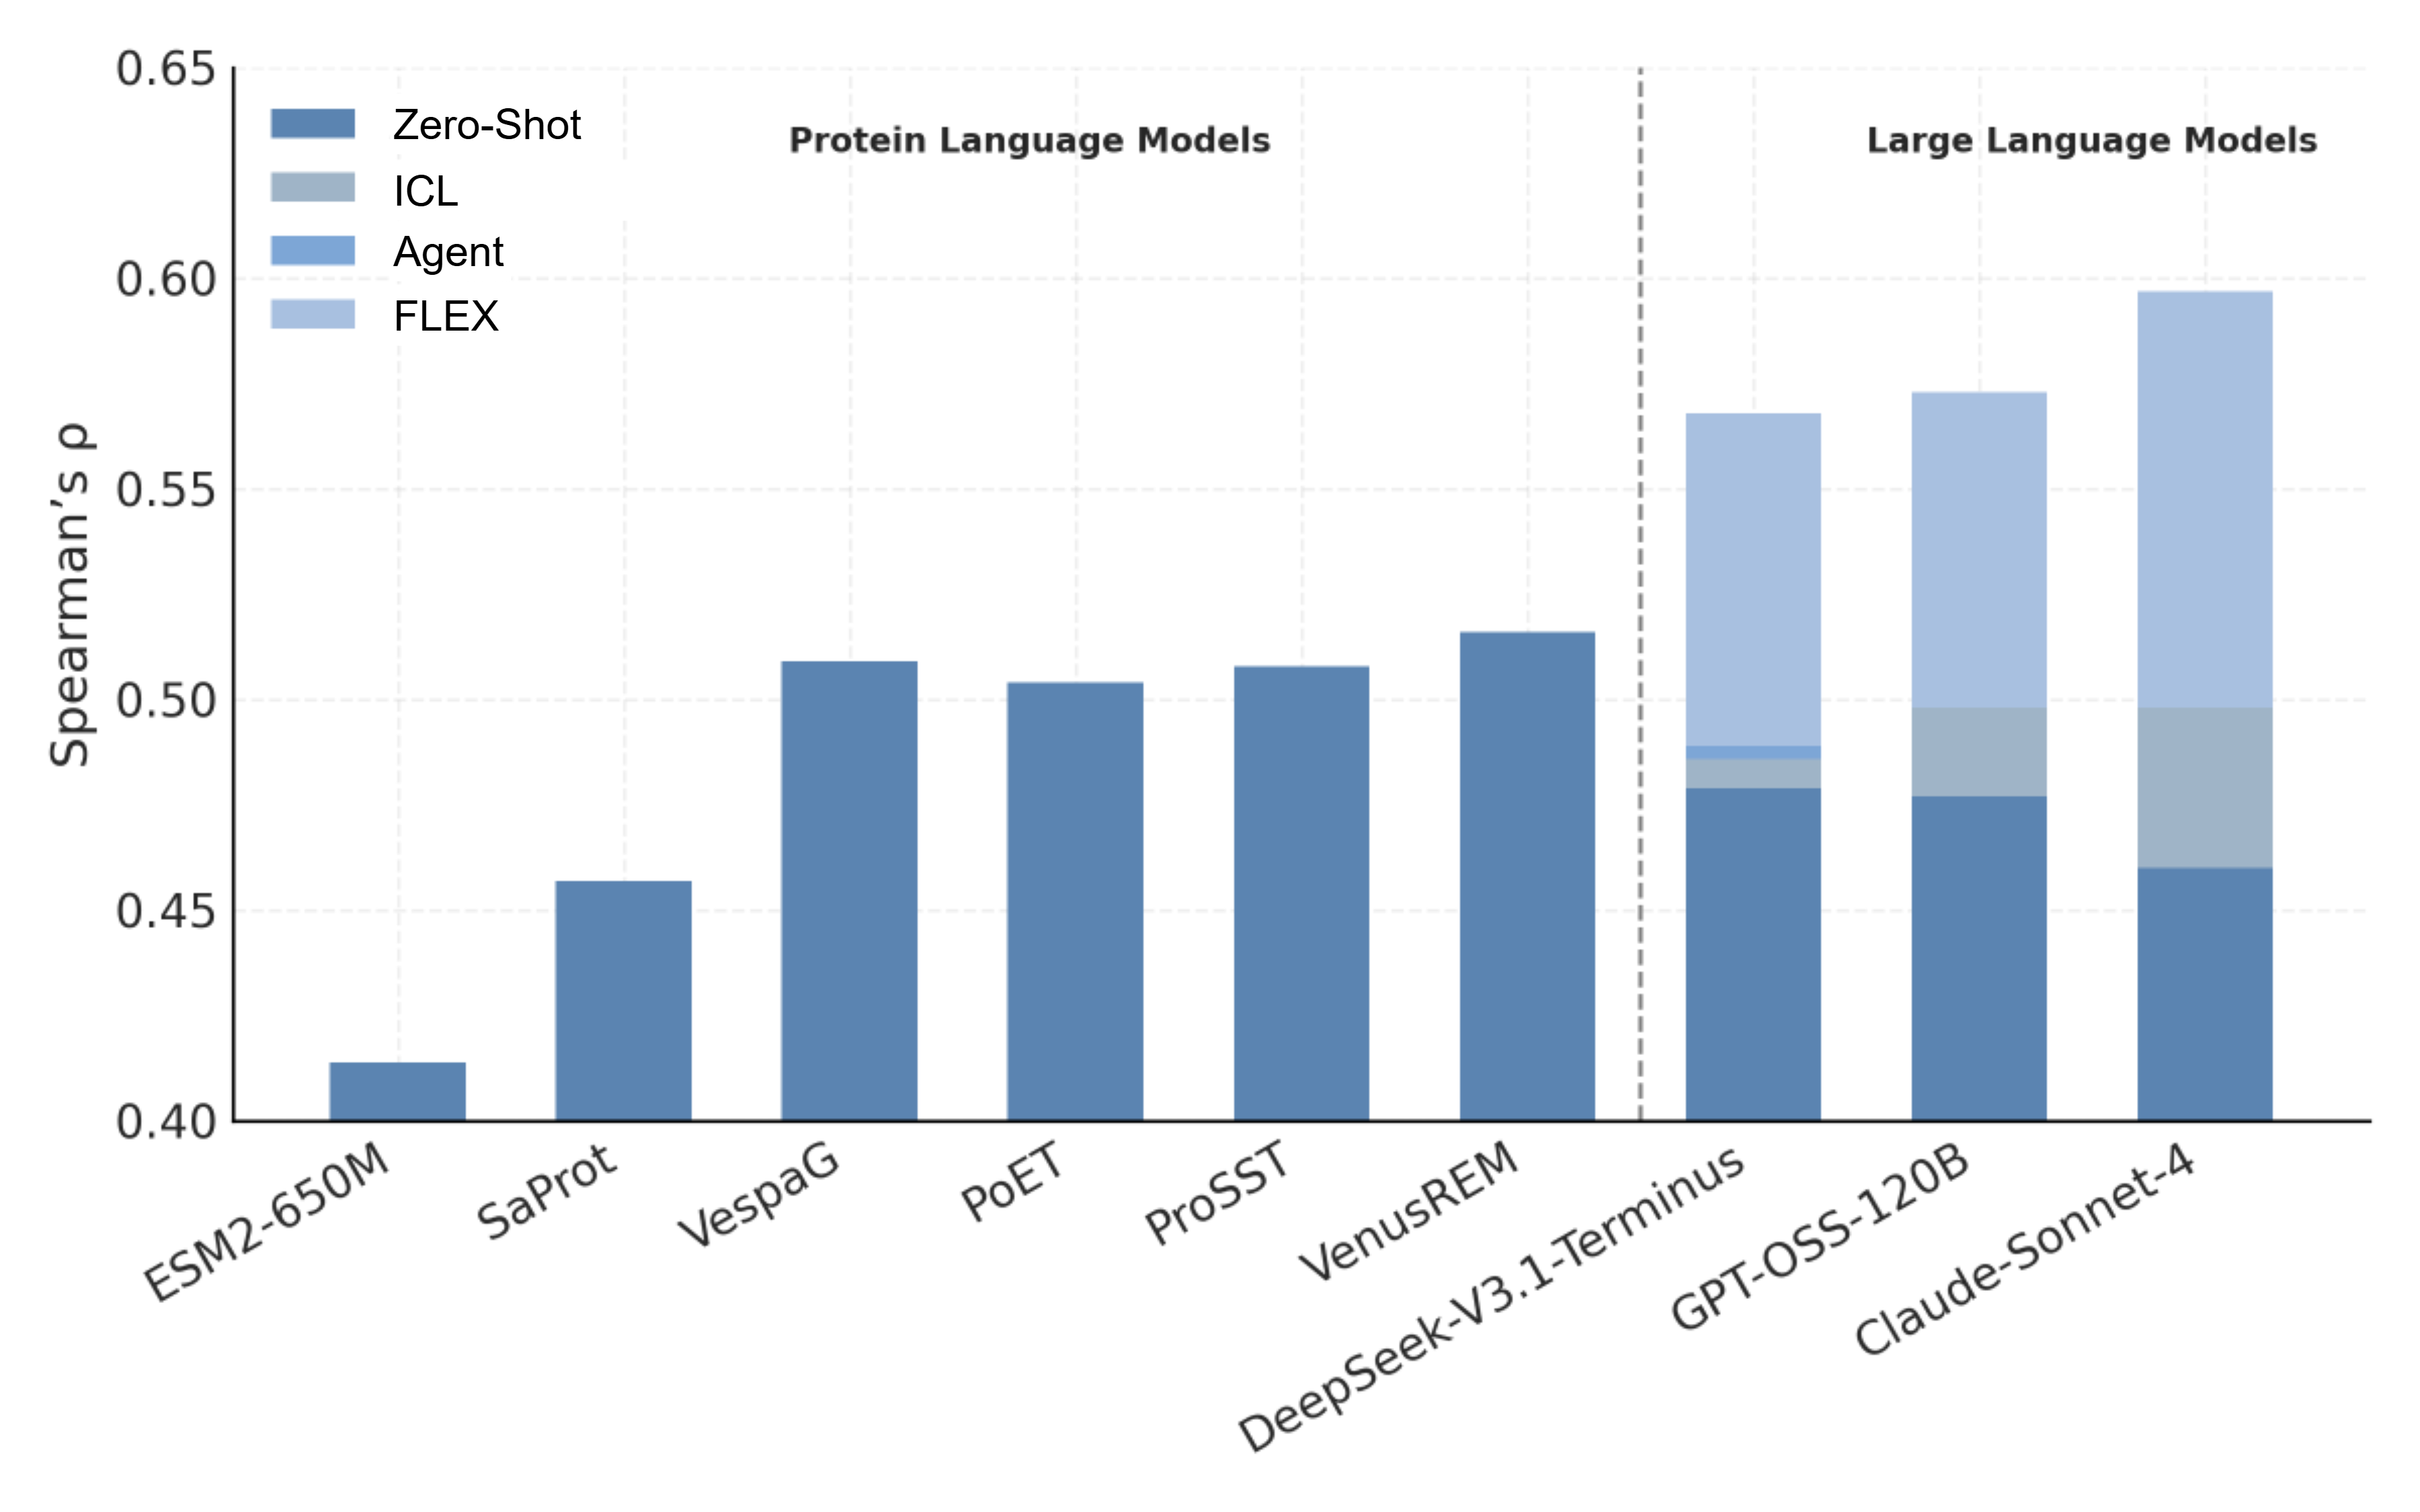
\includegraphics[width=0.98\linewidth]{./figs/proteingym_all.png}
  \caption{ProteinGym Results from both protein language model and large language model.}
  \label{fig:proteingym_all}
\end{figure}


\paragraph{Setup.} Prediction performance is evaluated using the Spearman rank correlation between the ground truth DMS (deep mutational scanning) scores and the proxy metrics generated by our \method{} method. Baseline models are grouped into two main categories:

\textit{Zero-shot Protein Fitness Prediction Models.} These models represent the current state-of-the-art on the ProteinGym leader-board and provide diverse biological priors through different input modalities:
\begin{itemize}
    \item VespaG~\cite{marquet2024expert, marquet2022embeddings}: A top-performing single-sequence model leveraging PLM embeddings and evolutionary guidance from GEMME~\cite{laine2019gemme}.
    \item PoET~\cite{truong2023poet}: A homolog-based model that encodes multiple sequence alignments using a sequence-of-sequences transformer architecture.
    \item ProSST~\cite{li2024prosst}: A hybrid model incorporating structural quantization and disentangled attention mechanisms to jointly model sequence and structural representations.
    \item VenusREM~\cite{tan2025high}: The current state-of-the-art on the ProteinGym scoreboard, integrating logits from single-sequence, homology, and structural tokenization signals.
\end{itemize}
These models provide the input features that our agent uses to reason about and construct enhanced fitness metrics.

\textit{Native Large Language Models (LLMs).} To isolate the contribution of agentic reasoning, we evaluate several high-performance LLMs—such as GPT-OSS~\cite{agarwal2025gpt} and Claude-Sonnet-4.5 as direct baselines. These models are prompted to perform the same prediction task as our forward learning system but without employing experience validation, rejection sampling and refinement. This comparison highlights the added value of structured forward learning beyond raw language model capabilities.

% \textbf{Main Results.} As illustrated in Table \ref{tab:main_table} and Figure \ref{fig:proteingym_all}, native LLMs fails on the task of importance selection and combination, with performance left behind of one single SOTA PLM as input. However, the incapability is levitated by forwarding learning paradigm. With experience extracted from a small validation set, learn golden rules and valuable lessons could be applied to bigger and wider test set with huge performance boost. In addition, instead of coming up with idea of formula with LLM itself, assistant of light-weight regression tools may also beneficial to this task.

\begin{table}[t!]
\centering
\caption{Ablation study results in ProteinGym benchmark of forward learning paradigm component techniques: \textbf{Experience Exploration}, \textbf{Experience Evolution}, \textbf{Assistance of Regression tools}. Where Fixed mean best one for all regression tools is used instead of each different regression tools for protein target selected by agent.}
\label{tab:proteingym_ablation_matrix}

\resizebox{\textwidth}{!}{%
\begin{tabular}{ccccc}
\toprule
\textbf{Model} & \textbf{Experience Exploration} & \textbf{Experience Evolution} & \textbf{Regression Tools} & \textbf{Spearman's $\rho$} \\
\midrule
\multirow{7}{*}{GPT-OSS}
& \xmark & \xmark & \xmark & 0.472 \\
& \xmark & \xmark & Fixed & 0.531 \\
& \cmark & \xmark & \xmark & 0.537 \\
& \xmark & \cmark & \xmark & 0.547 \\
& \cmark & \cmark & \xmark & 0.573 \\
& \cmark & \cmark & Fixed & 0.568 \\
& \cmark & \cmark & \cmark & \textbf{0.581} \\
\bottomrule
\end{tabular}
} % end of resizebox
\end{table}


\textbf{Ablation Study.} From Table \ref{tab:proteingym_ablation_matrix} we can learn that, three core parts of our \method{} paradigm contributed to performance enhancement: Experience Exploration, Experience Evolution, Regression Tools. Specificlly, Experience Exploration provide success and failure cases agent used to engage to, in the ProteinGym Scenario, common features included in most successful cases suggest its effect-ness in prediction final proxy metric. Experience Evolution enables agent to summarize past experience, update lessons learned recently with new cross-validation facts. Moreover, based on accurate selection of top importance features, regression tools could help agents to further adjust limited hyper-parameters, where deciding what kinds of regression works best still important for agents compared to the fix, one for all regression cases.








% \textbf{Case Study.} Figure \ref{fig:case_study} provides an example of how agents learn from a deliberately designed experience library—golden rules, warnings, and core know-how. Unlike the math and retro-synthesis problems above, protein-fitness prediction rarely admits absolute right/wrong answers; instead, useful guidance must be distilled from empirical trial trajectories and cross validation signals. The library captures those trajectories as reusable micro-strategies and failure patterns, enabling the agent to adapt a generic regression objective to the idiosyncrasies of a specific protein. In practice this means shifting attention away from globally renowned, aggregate metrics toward complementary, target-specific features and modeling choices that actually improve performance on the individual proteins.
% Moreover, the distilled tips actively drive algorithmic evolution: they suggest pre-processing pipelines, feature-combination heuristics, and validation gates that make final formula more robust. By overlaying proven procedural scaffolds onto the frozen LLM’s heuristic search, the experience library encourages more valuable and diverse explorations and simultaneously enlarges meaningful solutions that better tuned to the peculiarities scenarios.
